\documentclass[11pt]{article}
\usepackage{charter}
\usepackage{graphicx}
\usepackage{hyperref}
\usepackage[margin=1in]{geometry}
\usepackage{amsmath}

\hypersetup{
	colorlinks=true,
	linkcolor=blue,
	filecolor=magenta,
	urlcolor=cyan,
}

\begin{document}

%===================================================
% Title and Author Info
%===================================================
\begin{center}
{\Large\textsc{Newtonian Tidal Effects and Neutron Star Inspiral}} \\
\vspace{10pt}
{\large \textbf{Mentor:} Alex Urban} \\
{\small LIGO Laboratory, California Institute of Technology \\
Pasadena, CA 91125, USA \\
\href{mailto:aurban@ligo.caltech.edu}{\texttt{aurban@ligo.caltech.edu}}}
\end{center}

\section*{Purpose}

\hspace{15pt} In this problem, we will bring together a couple of basic things we know about orbits and make a toy model of a binary neutron star system. The goal is to use what we understand now to inform what we're going to do next: with nothing more than Kepler's laws and Newton's law of gravity, we will build an intuition for what happens just before a pair of neutron stars spiral into one another, and use those insights to strategize the next step.... \textit{of science!}

\section*{A De-Complicated Toy Model}
\hspace{15pt} Suppose that a neutron star binary (each with mass $M = 1.4\,\, M_{\odot}$) is in a stable, Keplerian orbit (\textit{i.e.} with no loss of energy). Figure \ref{fig:binary_diagram} illustrates this system.

\begin{enumerate}
\item Compute the separation (in km) between the stars in terms of the gravitational wave frequency.

\item Compute the gravitational force between star 1 and a chunk of mass on the near side of star 2, and again for a chunk on the far side of star 2. Compare this, quantitatively, to the gravitational self-force binding star 2 together, and make a plot of these quantities \textit{vs}. the gravitational wave frequency.”
\end{enumerate}

\vspace{30pt}

\begin{figure}[!h]
\centering
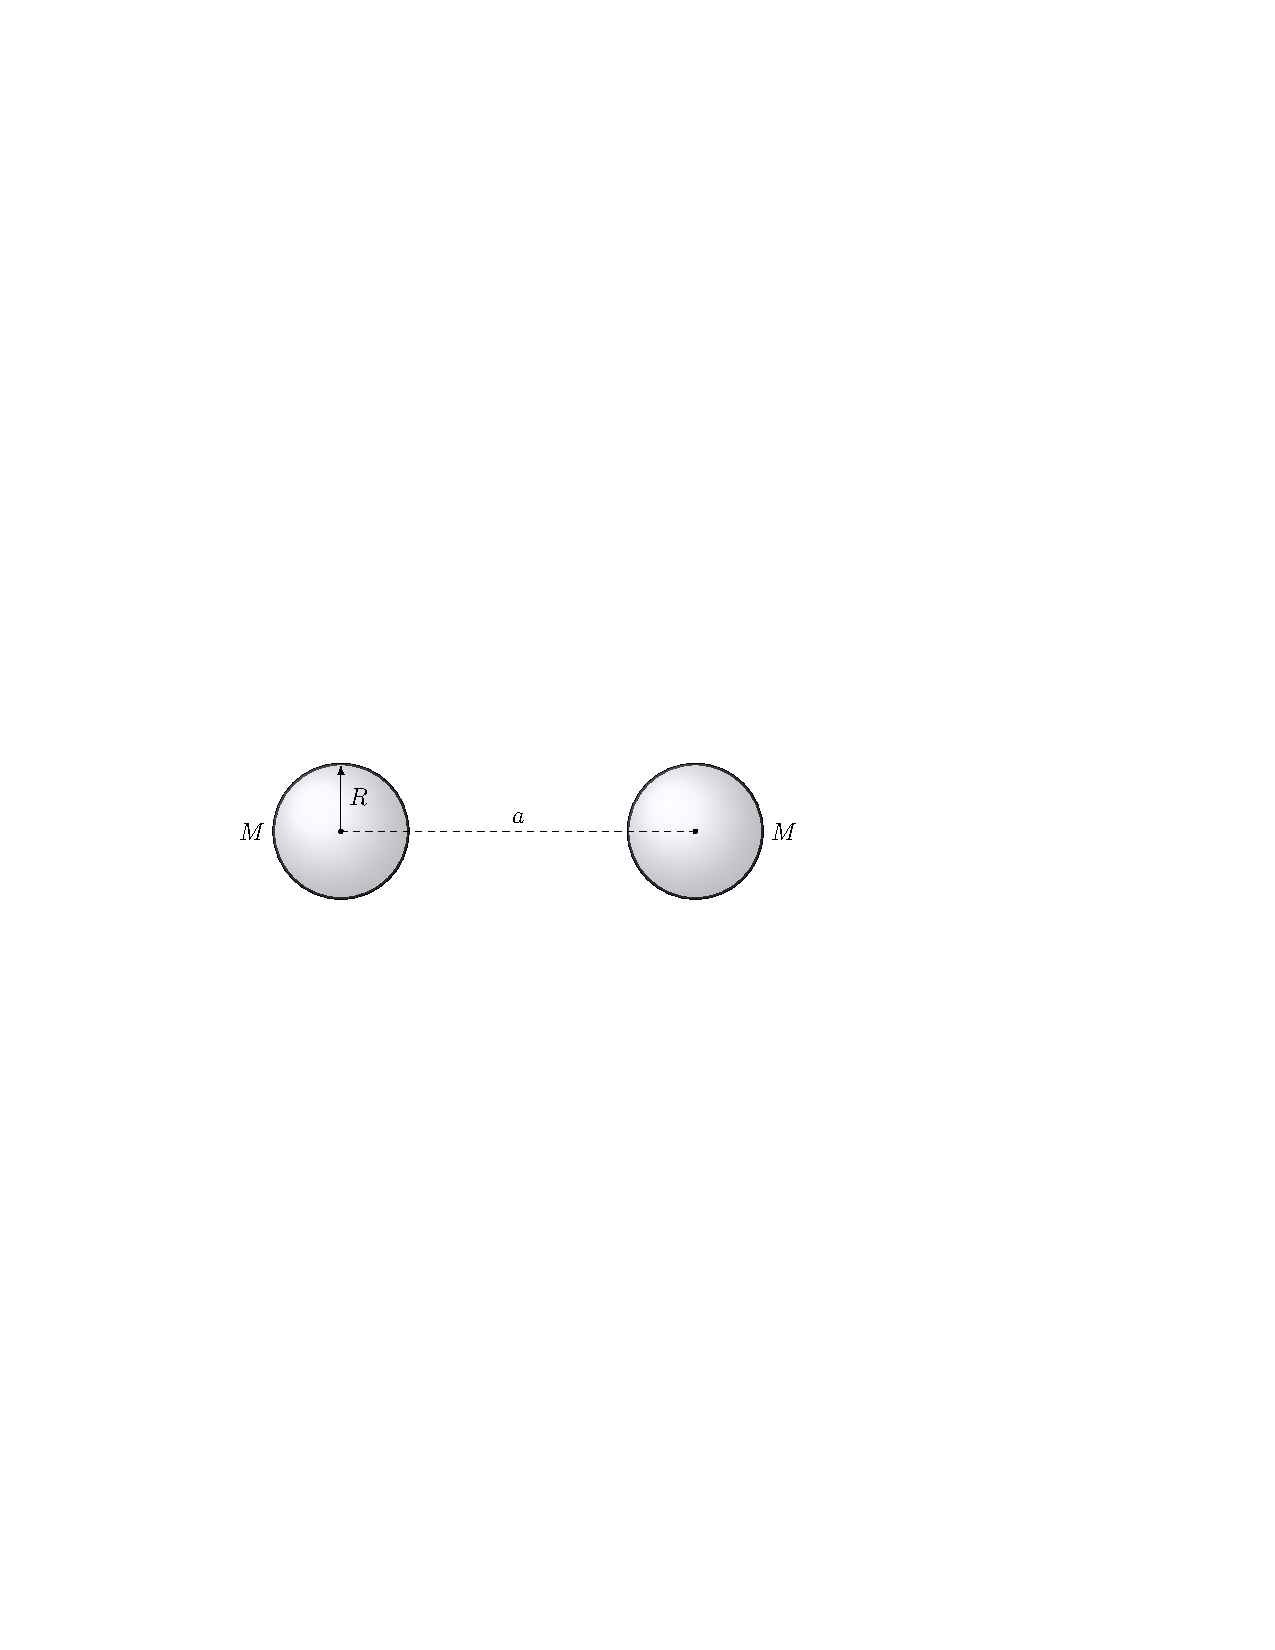
\includegraphics{binary_diagram.pdf}
\caption{\label{fig:binary_diagram}Diagram of the neutron star binary, showing its orbital separation ($a$) and the radius ($R$) and masses ($M$) of the individual neutron stars. The various mutual gravitational forces at play are also illustrated.}
\end{figure}

\vspace{1000pt}

\subsection*{Solution}

\hspace{15pt} Here's my attempt at a straightforward solution:

\begin{enumerate}

\item From Kepler's third law we can relate the orbital period ($P_{\rm orbital}$) and the orbital separation ($a$):
\[
\frac{P^2_{\rm orbital}}{a^3} = \frac{4\pi^2}{2GM}.
\]
Based on the symmetry of the orbit, we also know that gravitational waves will radiate from this system at twice the orbital frequency, $f_{\rm GW} = 2f_{\rm orbital} = 2/P_{\rm orbital}$. So, we can solve for $a$ in terms of $f_{\rm GW}$ with a bit of algebra:
\begin{equation}
a = \left[ \frac{2GM}{(\pi f_{\rm GW})^2} \right]^{1/3}.
\end{equation}

\item From Newton's law of gravitation, we know that the force felt by star 2 due to star 1 on its near side (see Figure \ref{fig:binary_diagram}) is
\begin{equation}
F_{\rm near} = \frac{GM^2}{(a - R)^2}
\end{equation}
where $R$ is the neutron star radius and the force vector points toward star 1. Similarly, the force felt on the far side is
\begin{equation}
F_{\rm far} = \frac{GM^2}{(a + R)^2}
\end{equation}
toward star 1. The difference between these is the tidal force:
\begin{equation}
F_{\rm tidal} = F_{\rm near} - F_{\rm far} = GM^2 \left( \frac{1}{(a - R)^2} - \frac{1}{(a + R)^2} \right).
\end{equation}
When the tidal force overcomes the gravitational self-force that binds star 2 together,
\begin{equation}
F_{\rm self} = \frac{GM^2}{R^2}
\end{equation}
(toward the center of star 2), we know this neutron star will start to be utterly demolished. Figure \ref{fig:NS_tides} illustrates this process for different neutron star radii, in terms of the gravitational wave frequency.

\end{enumerate}

\begin{figure}
\centering
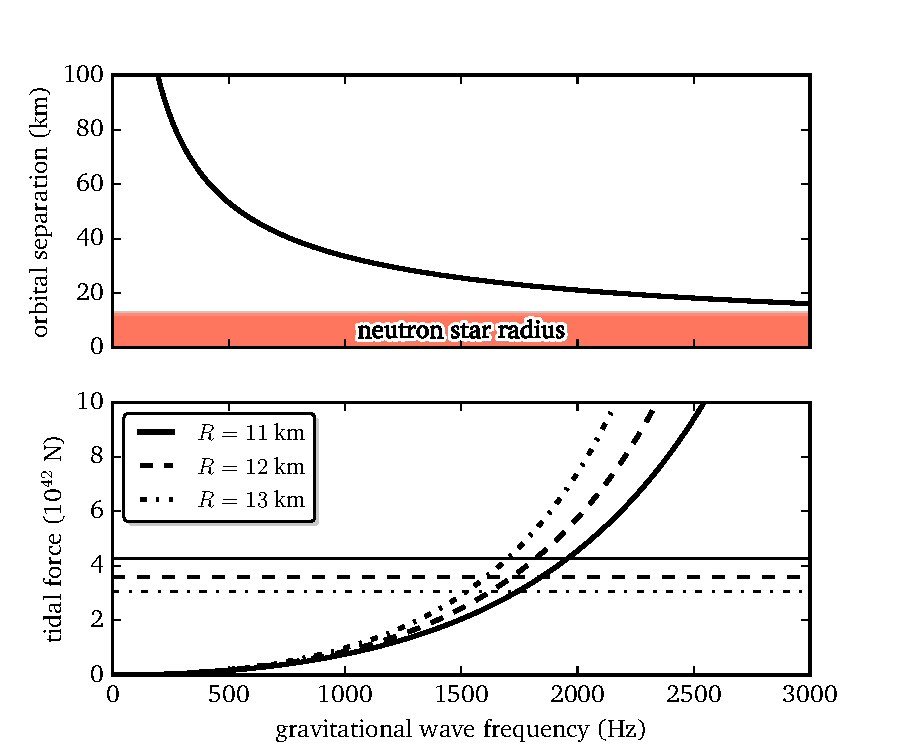
\includegraphics[scale=1]{newtonian_tidal_forces.pdf}
\caption{\label{fig:NS_tides}Top: the orbital separation (in km) between two neutron stars as a function of gravitational wave frequency. Bottom: The tidal force (in Newtons) on one neutron star due to the pull of the other, compared at different neutron star radii. The horizontal lines show the neutron star's total self-binding force -- when the tidal force overcomes this, the neutron star will be ripped to smitherines in an absolutely \emph{epic} lightshow.}
\end{figure}

\section*{Things That Make You Go, ``Hmmm....''}

\begin{enumerate}

\item Of course, Newton's third law of motion guarantees that any gravitational action between the two neutron stars will be felt mutually. Given this, can you paint a qualitative picture of tidal deformation?

\item Tidal forces are still very important even in non-extreme gravitational fields, such as between the Moon and Earth. Can you show that $F_{\rm tidal} \propto 1/a^3$ when $R/a$ is small? Hint: use the Maclaurin series!

\end{enumerate}

\section*{Next Steps}

\hspace{15pt} Having understood all this, we now want to want to polish a different skill that will be necessary later: numerical modeling. Can you think of a toy model that would be easy to simulate in Python?

\end{document}
